\documentclass[main.tex]{subfiles}
\begin{document}

\section{Hardware}

With the increasing demand for highly data-parallel algorithms, and the increasing amount of data to process, hardware development started shifting towards the goal of solving that problem. Initially, that started with the increased support for vector instructions in common \acsp{CPU}, and the \acs{SIMD} model. This allowed a single instruction to operate on a set of elements at once, effectively achieving a kind of parallelism which was extremelly useful with highly data-parallel applications. Modern \intel processors, starting with the Sandy Bridge family, already support \ac{AVX} \todo{refs refs refs}, an extension to the \textit{x86} instruction set allowing \acs{SIMD} instructions capable of handling 256 bits registers. This extension also introduces three-operand \acs{SIMD} instructions that allow more general $c = a + b$ operations to be handled with a single instruction, in addition to the previous instructions which only allowed two operands ($a = a + b$).

\acs{SIMD} is also the programming model behind \acsp{GPU}, which gradually started to gain more attention for their general purpose computing capabilites. Although the hardware of a \acs{GPU} is still tightly coupled with graphics processing and rendering, there have also been several advances in their usage as \acp{GPGPU}.


%%%%%%%%%%%%%%%%%%%%%%%%%%%%%%%%%%%%%%%
\subsection{\nvidia Fermi Architecture}

The Fermi architecture was an important milestone of \acs{GPU} technology, as it was one of the first generations target directly towards \acs{GPGPU} and high performance computing, rather than just graphics rendering. The first Fermi devices were released in 2010, and were the first \nvidia products to include support for double precision floating point number, which was an important feature for high performance computing to provide more accurate results. Fermi devices also included a GDDR5 memory controller with support for \ac{DMA} through the \acs{PCI-e} bus, and up to 16 \acf{SM}, for a total of up to 512 \acs{CUDA} Cores.

Each \ac{SM} has a total of $64KB$ of private memory available, which can be configured to be split between Shared Memory and L1 cache, although configuration was restricted to either $48KB + 16KB$ or $16KB + 48KB$. This provided some flexibility to the devices, since some problems would benefit more from the extra Shared memory and not so much from cache, and vice-versa.

Additionally, all \acsp{SM} share a common $768KB$ L2 cache, and a final level of global memory, that can go up to 6GB of GDDR5, with a bandwidth of 192.6 GB/s in the Tesla C2070 \cite{NVIDIA:fermi}.

\begin{figure}[!htp]
  \centering
  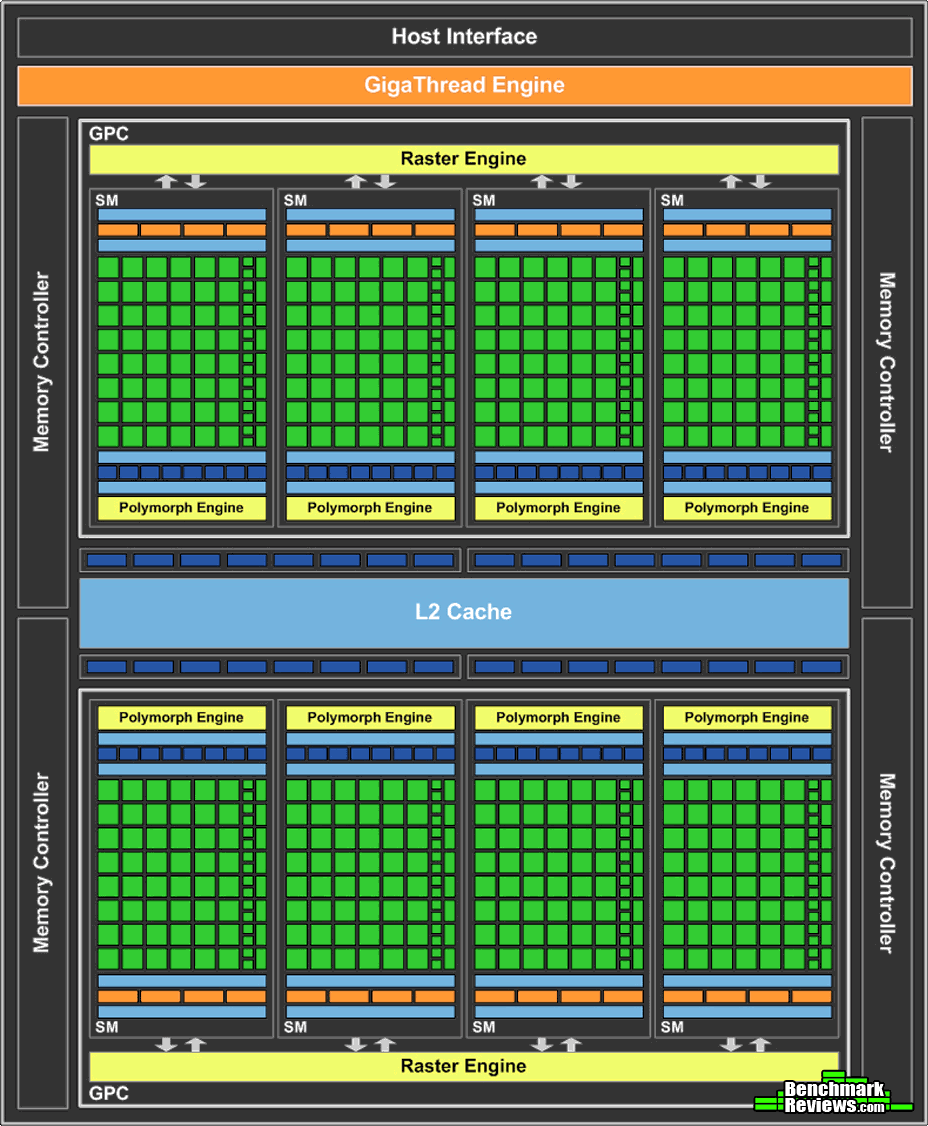
\includegraphics[width=0.4\textwidth]{arch_fermi}
  \caption{Overview of the Fermi architecture \label{fig:fermi}}
\end{figure}

This architecture is backed by a hardware-based thread scheduler, located within each \acs{SM}, that attempt to feed the execution unit with threads grouped in blocks of 32, or \textit{warps}. All threads within a warp are considered to be independent from each other, so there is no need for dependency checking. Any thread that is waiting for memory accesses to be finished will remain unscheduled until the required data is available. Since the scheduling is made directly via hardware, the switch between threads is nearly free, at least when compared with thread scheduling on a \acs{CPU}. As a result, this strategy works better when the total amount of threads competing for resources is much higher than the amount of execution units, allowing for the latency of memory accesses to be hidden away by instanly scheduling a different \textit{warp}, effectively hiding memory latency while still keeping execution units busy. This is very different from \acs{CPU} scheduling policies, where switching between threads requires a switch of context, a takes considerably more time, making that approach not as viable as for a \acs{GPU}.



&%%%%%%%%%%%%%%%%%%%%%%%%%%%%%%%%%%%%%%%
\subsection{\nvidia Kepler Architecture}

The follow-up generation to Fermi is in many ways similar to its predecessor. One of the most notorious change is the increase in the total amount of \acs{CUDA} Cores available, capable of going up to 2880 in high-end devices, due to the new redesign of \acl{SM} which was named \acs{SMX}, each one featuring 192 \acs{CUDA} Cores.

Memory was also upgraded over the previous generations, wiht the maximum amount of registers going from 63 to 255, the addition of an extra $48KB$ L1 read-only cache, while still maintaning the original L1 cache, and L2 cache going up to a maximum of $1.5MB$ with increased bandwidth \cite{NVIDIA:kepler}.

The programming model has been extended with the addition of Dynamic Parallelism, allowing \acs{CUDA} thread to spawn new threads, a feature not possible with previous versions. This is an important feature for irregular algorithms, such as Ray Tracing or graph based problems.

\begin{figure}
  \centering
  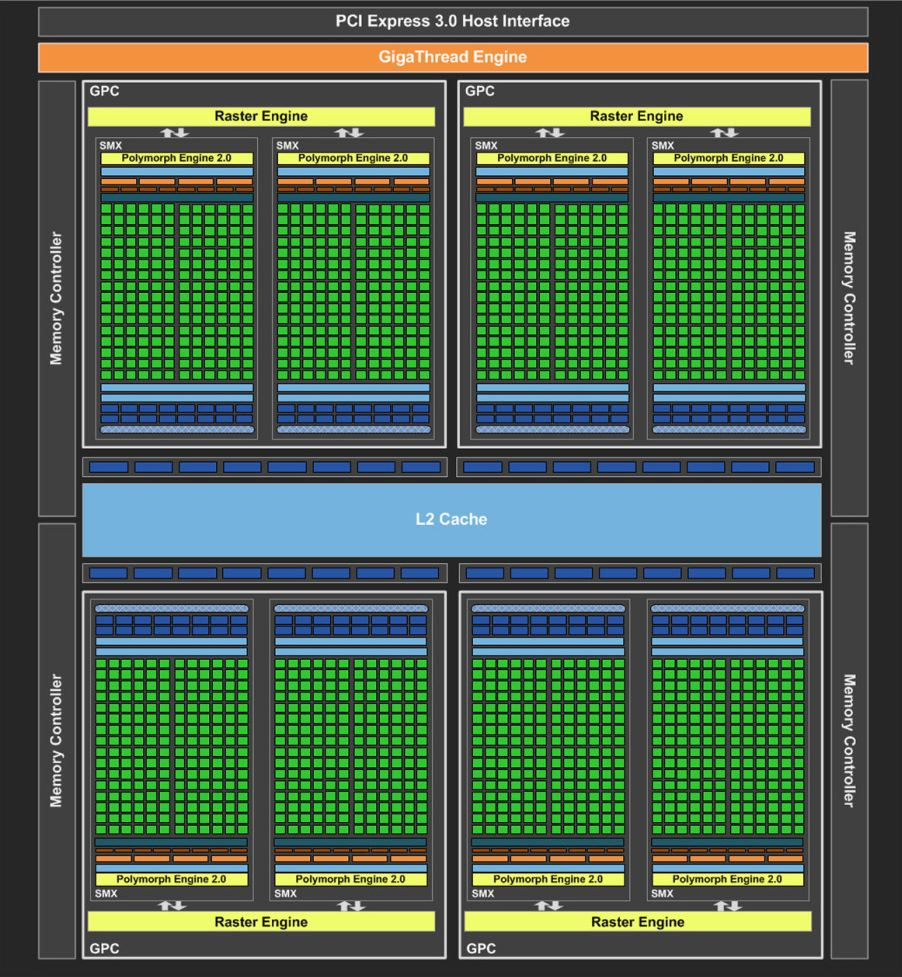
\includegraphics[width=0.4\textwidth]{arch_kepler}
  \caption{Overview of the Kepler architecture \label{fig:kepler}}
\end{figure}



\subsection{\intel Many Integrated Core}


\end{document}
